\documentclass[10pt]{article}

\usepackage{amsmath, amssymb}
\usepackage[margin=1in]{geometry}
\usepackage{enumitem}
\usepackage{tikz}
\usetikzlibrary{shapes.geometric, backgrounds, calc}
\usepackage{calc}
\usepackage{multicol}

\usepackage{xcolor}
\definecolor{color1}{RGB}{0, 99, 178} % Electric Blue Lemonade
\definecolor{color2}{RGB}{193, 228, 242} % Sky Blue

\setlength{\parskip}{1ex}
\setlength{\parindent}{0pt}

\newlength{\topedge}
\newlength{\bottomedge}

% Section styling
\usepackage{titlesec, titletoc}
\titleformat{\section}[display]{}{}{0pt}{
    \bf \Large \color{white}
    \setlength{\topedge}{0.9\baselineskip}
    \setlength{\bottomedge}{-0.4\baselineskip}
    \begin{tikzpicture}[overlay, x=1in, y=1in]
        \fill[color1] (-1, \bottomedge) -- (6.5, \bottomedge) -- (6.2, \topedge) -- (-1, \topedge) -- cycle;
    \end{tikzpicture}%
}[]
\titlespacing*{\section}{0pt}{-3ex}{1ex} % remove some space before, add some after

% Subsection styling
\titleformat{\subsection}[display]{}{}{0pt}{
    \bf \large \color{white}
    \setlength{\topedge}{0.9\baselineskip}
    \setlength{\bottomedge}{-0.4\baselineskip}
    \begin{tikzpicture}[overlay, x=1in, y=1in]
        \fill[color1] (-1, \bottomedge) -- (2.75, \bottomedge) -- (2.5, \topedge) -- (-1, \topedge) -- cycle;
    \end{tikzpicture}%
}[]
\titlespacing*{\subsection}{0pt}{-2ex}{0pt} % remove some space before

\usepackage{pgfplots}
\pgfplotsset{
    disabledatascaling,
    cycle list=black, 
    axis lines=middle,
    every axis plot/.style={no marks, thick},
    every axis/.style={
        enlarge x limits=false,
        enlarge y limits=auto,
        xlabel style={at={(current axis.right of origin)},anchor=west},
        ylabel style={at={(current axis.above origin)},anchor=south},
        % extra x and y ticks for asymptotes
        extra x tick style={grid=major, grid style={dashed,black}},
        extra y tick style={grid=major, grid style={dashed,black}},
        /pgf/number format/1000 sep={},
    },
    tick label style = {font=\footnotesize, inner sep=0pt},
    xticklabel shift=1pt,    
    scaled ticks=false,
    scaled y ticks=false,
    unbounded coords=jump,
    samples=101,
    minor tick length=0,
    scatter/classes={
        open={mark=*,draw=black,fill=white, mark size=2, thin},
        closed={mark=*,draw=black,fill=black, mark size=2, thin}
    },
    width=3in,
}
\pgfplotsset{open/.style={only marks, mark=*, fill=white, thin}}
\pgfplotsset{closed/.style={only marks, mark=*, draw=black, fill=black, thin}}

\usepackage[colorlinks, linkcolor=color1, urlcolor=color1]{hyperref}

% change to \usepackage[sols,grading]{../Documents/handout} to see solutions/grading notes
\usepackage[]{../Documents/handout}

\usepackage{fdsymbol}
\setlist{itemsep=1ex, parsep=1ex, topsep=1ex}
\setlist[itemize]{label={\color{color1} $\smallblackdiamond$}}

% fancy enumeration
\DeclareRobustCommand{\numbox}[1]{\tikz[overlay, baseline=-10pt, trapezium stretches=true] \node[trapezium, trapezium left angle=45, trapezium right angle=90, shape border rotate=90, anchor=north, text depth=1cm, inner ysep=8pt, fill=color1, text=white, font=\Large]{#1}; \,}
\DeclareRobustCommand{\shortnumbox}[1]{\tikz[overlay, baseline=-10pt, trapezium stretches=true] \node[trapezium, trapezium left angle=45, trapezium right angle=90, shape border rotate=90, anchor=north, inner ysep=8pt, fill=color1, text=white, font=\Large]{#1}; \,}

\begin{document}

\begin{center}
    
\begin{tikzpicture}
        \node (title) [trapezium, trapezium left angle=60, trapezium right angle=120, align=center, inner sep=10pt, fill=color1, text=white] at (0, 0) {\bf \LARGE Modeling with Functions};
        \node[trapezium, trapezium left angle=120, trapezium right angle=60, align=center, inner sep=6pt, fill=color2, text=black]
        at ($(title.top left corner) + (0,0.2)$) {\large Problem Set 1};
        \node[trapezium, trapezium left angle=120, trapezium right angle=60, align=center, inner sep=6pt, fill=color2, text=black]
        at ($(title.bottom right corner) + (0,-0.2)$) {\large Due Wednesday, Sep.\ 10};
    \end{tikzpicture}
\end{center}

\begin{problemonly}
    \vspace*{-0.8cm}
    \begin{center}
        \hspace*{-1in}
        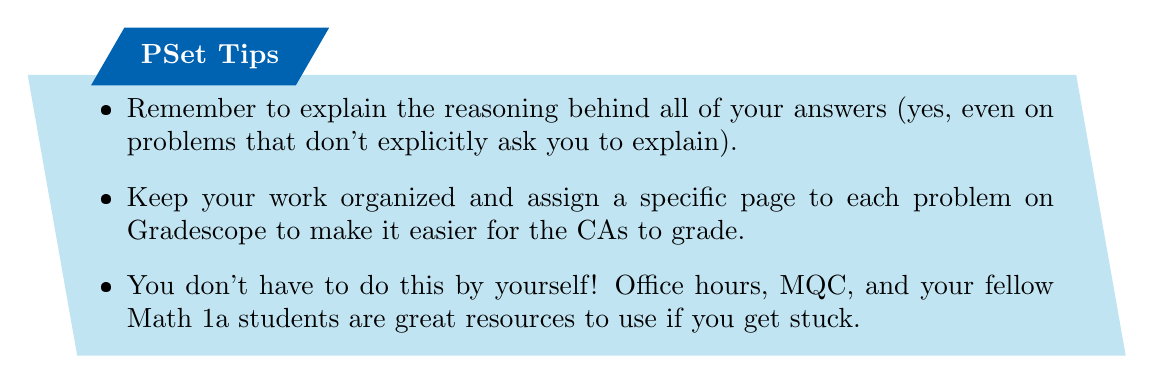
\begin{tikzpicture}
            \node (goals) [trapezium, trapezium left angle=100, trapezium right angle=80, align=center, inner sep=8pt, fill=color2, text=black] at (0, 0)
                {\begin{minipage}{\textwidth}
                    \begin{itemize}[leftmargin=*]
                        \item Remember to explain the reasoning behind all of your answers (yes, even on problems that don't explicitly ask you to explain).
                        \item Keep your work organized and assign a specific page to each problem on Gradescope to make it easier for the CAs to grade.
                        \item You don't have to do this by yourself! Office hours, MQC, and your fellow Math 1a students are great resources to use if you get stuck.
                    \end{itemize}
                \end{minipage}};
                
            \node[trapezium, trapezium left angle=60, trapezium right angle=120, align=center, anchor=bottom left corner, inner sep=6pt, fill=color1, text=white] at ($(goals.top left corner) + (0.8, -0.15)$) {\bf PSet Tips};
        \end{tikzpicture}
        \hspace*{-1in}
    \end{center}
\end{problemonly}

\begin{enumerate}[leftmargin=*, label=\numbox{\arabic*}]
\item[\refstepcounter{enumi}\shortnumbox{\number\value{enumi}}]
    \begin{problem}
        Jenkins is participating in a bike race; the course goes up a steep
        hill, so, as he rides, he goes more and more slowly.  Let $d(t)$ be
        the distance Jenkins has traveled (in meters) $t$ seconds into the
        race.  Is $d$ increasing or decreasing?  Concave up or concave down?
        Explain how you know.
    \end{problem}

    \begin{solution}
        Jenkins is always traveling during the race, so the distance $d$
        traveled increases as time goes on.  We're also told that he travels
        more slowly as time goes on, so the graph of $d$ is concave down.
    \end{solution}
\begin{grading}
2 points, one for pointing out that the distance increases, and the other for the concavity. If students do not justify their answers, give 1.5 points. 
\end{grading}
\item
    One of the best ways to make sure you understand mathematical
    properties like concavity is to play around with making examples with
    different properties.  That's what you'll do in this problem. \textbf{For the following parts of the problem, please give both a formula and a graph of your function.}

    \begin{enumerate}
        \item
        \begin{problem}
            Give an example of a function whose graph is decreasing and concave
            down on $(-\infty, \infty)$.  
        \end{problem}

        \begin{solution}
            There are infinitely many possible answers; one is a vertical flip
            (over the $x$-axis) of $e^x$, or $\boxed{-e^x}$.
        \end{solution}
    \begin{grading}
    2 points - 1 point for the function being decreasing, another for the concavity. Give 1.5 points if they draw or describe their function without giving an explicit formula, or if their formula is incorrect but their picture is correct.
    \end{grading}
        \item
        \begin{problem}
            Give an example of a function whose graph is increasing and concave
            down on $(0, \infty)$ and which passes through the points $(1, 1)$
            and $(2, 3)$.
        \end{problem}

        \begin{solution}
            Again, there are infinitely many possible answers.  One idea is to
            start with $\ln x$, which is increasing and concave down on $(0,
            \infty)$, and then stretch it vertically and shift it vertically so
            that it goes through the points $(1, 1)$ and $(2, 3)$.  (A vertical
            stretch and shift won't change the fact that the function is
            increasing and concave down on $(0, \infty$).)  A vertical stretch
            and shift of $\ln x$ has the form $f(x) = A \ln x + B$, and we're
            trying to find appropriate values of $A$ and $B$.
            
            In order to have $y = A \ln x + B$ go through the points $(1, 1)$
            and $(2, 3)$, we want $1 = A \ln 1 + B = B$ and $3 = A \ln 2 + B$.
            The first equation says that $B = 1$; plugging this into the second
            equation, $3 = A \ln 2 + 1$, so $A = \frac{2}{\ln 2}$.  Therefore,
            $\boxed{\frac{2}{\ln 2} \ln x + 1}$ is one example.  (This can be
            written more simply as $2 \log_2 x + 1$.)
        \end{solution}

        \begin{grading}
        4 points. 2 points for coming up with a function that is increasing and concave down on $(0, \infty)$, and then 2 points for setting up and solving the equations to have the function go through $(1, 1)$ and $(2, 3)$. 
        \end{grading}
    \end{enumerate}
    
\item
    In each part, give an example of a function $f$ satisfying the given
    properties. You should provide a formula and corresponding graph for $f(x)$. You may use technology (Desmos, Geogebra, etc) to come up with your graph. 
    (Try starting from a basic function you're familiar with and transforming to achieve the necessary properties.)
    
    \begin{enumerate}
        \item
        \begin{problem}
            A non-constant function $f$ with domain $(-\infty, \infty)$ such that $1.1 \leq f(x) \leq 1.3$ for all $x$.
        \end{problem}

        \begin{solution}
            One possibility is to use a sinusoid, something like this:
            \begin{center}
                \begin{tikzpicture}
                    \begin{axis}[xtick=\empty, ytick={1.1, 1.3}, ymin=0, width=3in, height=2in] 
                        \addplot+[domain=-10:10] {1.2 + 0.1*cos(deg(x))};
                    \end{axis}
                \end{tikzpicture}
            \end{center}
            We can use graph transformations to rescale (vertically) and shift; for a specific example, this is
            the graph of $\boxed{f(x) = 1.2 + 0.1 \cos x}$. 
        \end{solution}
        \begin{grading}
        3 points. 1 point for the function being bounded, 1 point for a correct formula for the function, 0.5 point for the function being defined and non-constant on the domain, 0.5 points for the graph. 
        \end{grading}

        \item
        \begin{problem}
            A function $f$ with domain $(2, \infty)$ which is always decreasing
            and which satisfies $f(5) = 4$.
        \end{problem}

        \begin{solution}
            The function $\ln x$ is a familiar function with domain $(0,
            \infty)$.  If we shift this 2 units to the right, then the domain of
            the shifted function will be $(2, \infty)$; that is, $\ln(x - 2)$
            has domain $(2, \infty)$.  This is an increasing function, but if we
            flip it over the $x$-axis, then we'll get a decreasing function.
            That is, $-\ln(x - 2)$ is a decreasing function with domain $(2,
            \infty)$.  Finally, we want to adjust our function so that $f(5) =
            4$; a simple way to do this is to shift it vertically.  So, we want
            a function of the form $f(x) = -\ln(x - 2) + A$ with $f(5) = 4$;
            that is, we want $-\ln(3) + A = 4$, so $A = 4 + \ln 3$.  Thus, one
            example is $\boxed{-\ln(x - 2) + 4 + \ln 3}$. 
        \end{solution}
        
        \begin{grading}
        4 points. 1 point for the function always decreasing on $(2, \infty)$, 1 point for the function going through the point, 1 point for correctly showing work/how they transform the base function, 0.5 points for the graph, 0.5 points for being defined on the full domain.
        \end{grading}
        \item
        \begin{problem}
            A function $f$ with domain $(-\infty, \infty)$ which is always
            decreasing and has the property that $f(x) > \pi$ for all $x$.
        \end{problem}

        \begin{solution}
            Graphically, we might picture a function like this:
            \begin{center}
                \begin{tikzpicture}
                    \begin{axis}[width=3in, height=2in, ytick=\empty, xtick=\empty, extra y ticks={3.14}, extra y tick labels={$\pi$}, ymin=0]
                        \addplot+[domain=-3:3] {pi + 2^-x};
                    \end{axis}
                \end{tikzpicture}
            \end{center}
            One possible formula for such a graph is $\boxed{f(x) = \pi + e^{-x}}$.
        \end{solution}
        \begin{grading}
        3 points. 0.5 points for graph, 0.5 points for function being defined on full domain, 1 point for being always decreasing on the domain, 1 point for having $f(x) > \pi$ for all $x$. 
        \end{grading}
        \item
        \begin{problem}
            A function $f$ with domain $(-\infty, \infty)$ where $f(2x) = 4 f(x)$ for all values of $x$. This takes a little playing around with basic functions, so don't be afraid to experiment. Please show a check that your formula actually works! (This means not just checking some points, but rather verifying algebraically).
        \end{problem}

        \begin{solution}
            A good strategy is to try using some of our basic functions, such as power functions. In this case, we see right away that $\boxed{f(x) = x^2}$ works: $f(2x) = (2x)^2 = 4 x^2 = 4 f(x)$. 
        \end{solution}
        \begin{grading}
        2 points. There should be a check that the function they propose actually works - if not, give 1.5 points.
        \end{grading}
    \end{enumerate}

\item
    \begin{problem}
        A band is trying to decide how to price tickets for its next concert.
        Their market research suggests that, if they price the tickets at \$20
        per ticket, then they will sell 1000 tickets.  For each \$2 increase
        in ticket price, the number of tickets they will sell decreases by 5.
        Write a formula for $R(p)$, the amount of money they will bring in from tickets if
        they price the tickets at $p$ dollars per ticket.
        \vspace{1ex}
        
        \textbf{Hint:} First try defining a function that represents the number of tickets they will sell per cost of $p$ dollars.
    \end{problem}

    \begin{solution}
        Let's start by defining the function $N(p)$, the number of tickets they will sell at a cost of $p$ dollars.
        $N(p)$ is a linear function because it changes at a constant rate of
        $\frac{-5 \text{ tickets}}{2 \text{ dollars}} = -2.5$ tickets per
        dollar.  In particular, its slope is $-2.5$; since its graph passes
        through the point $(20, 1000)$, the point-slope form of a line gives
        \begin{align*}
            N(p) - 1000 &= - 2.5 (p - 20) \\
            N(p) &= 1000 - 2.5 (p - 20)
        \end{align*}

        To determine the amount of money the band makes, we need to multiply the number of tickets $N(p)$ sold by the price $p$:
            $$\boxed{R(p) = p(1000 - 2.5(p-20))}$$
    \end{solution}
    \begin{grading}
    6 points. 2 points for recognizing that the number of tickets changes at a constant rate of $-2.5$, 2 points for using the point $(20, 1000)$ to find a correct formula for $N(p)$, and another 2 points for writing that $R(p)$ is $p$ times $N(p)$ (in whatever form they found for $N(p)$, even if it is incorrect). Give generous partial credit and note that students do not need to fully simplify their answers. 
    \end{grading}
\end{enumerate}

\end{document}